\documentclass{article}
\usepackage[utf8]{inputenc}
\usepackage[T1]{fontenc}
\usepackage[francais]{babel}
\usepackage{lmodern}
\usepackage{graphicx}
\usepackage{geometry}

\geometry{hmargin=30pt, vmargin=30pt}

\title{Schéma global du projet : Tableau virtuel interactif}
\author{Bollini Kevin, Mélia Geoffrey, Pagès Julien, Saleil Baptiste}

\begin{document}

\maketitle

\section{Introduction}
Ce document présente une présentation de notre projet, et un aperçu sur le fonctionnement de notre application.

\section{Schéma Global}
Le schéma ci dessous présente de façon globale les différents modules pour une utilisation en réseau de l'application.
	\begin{center}
	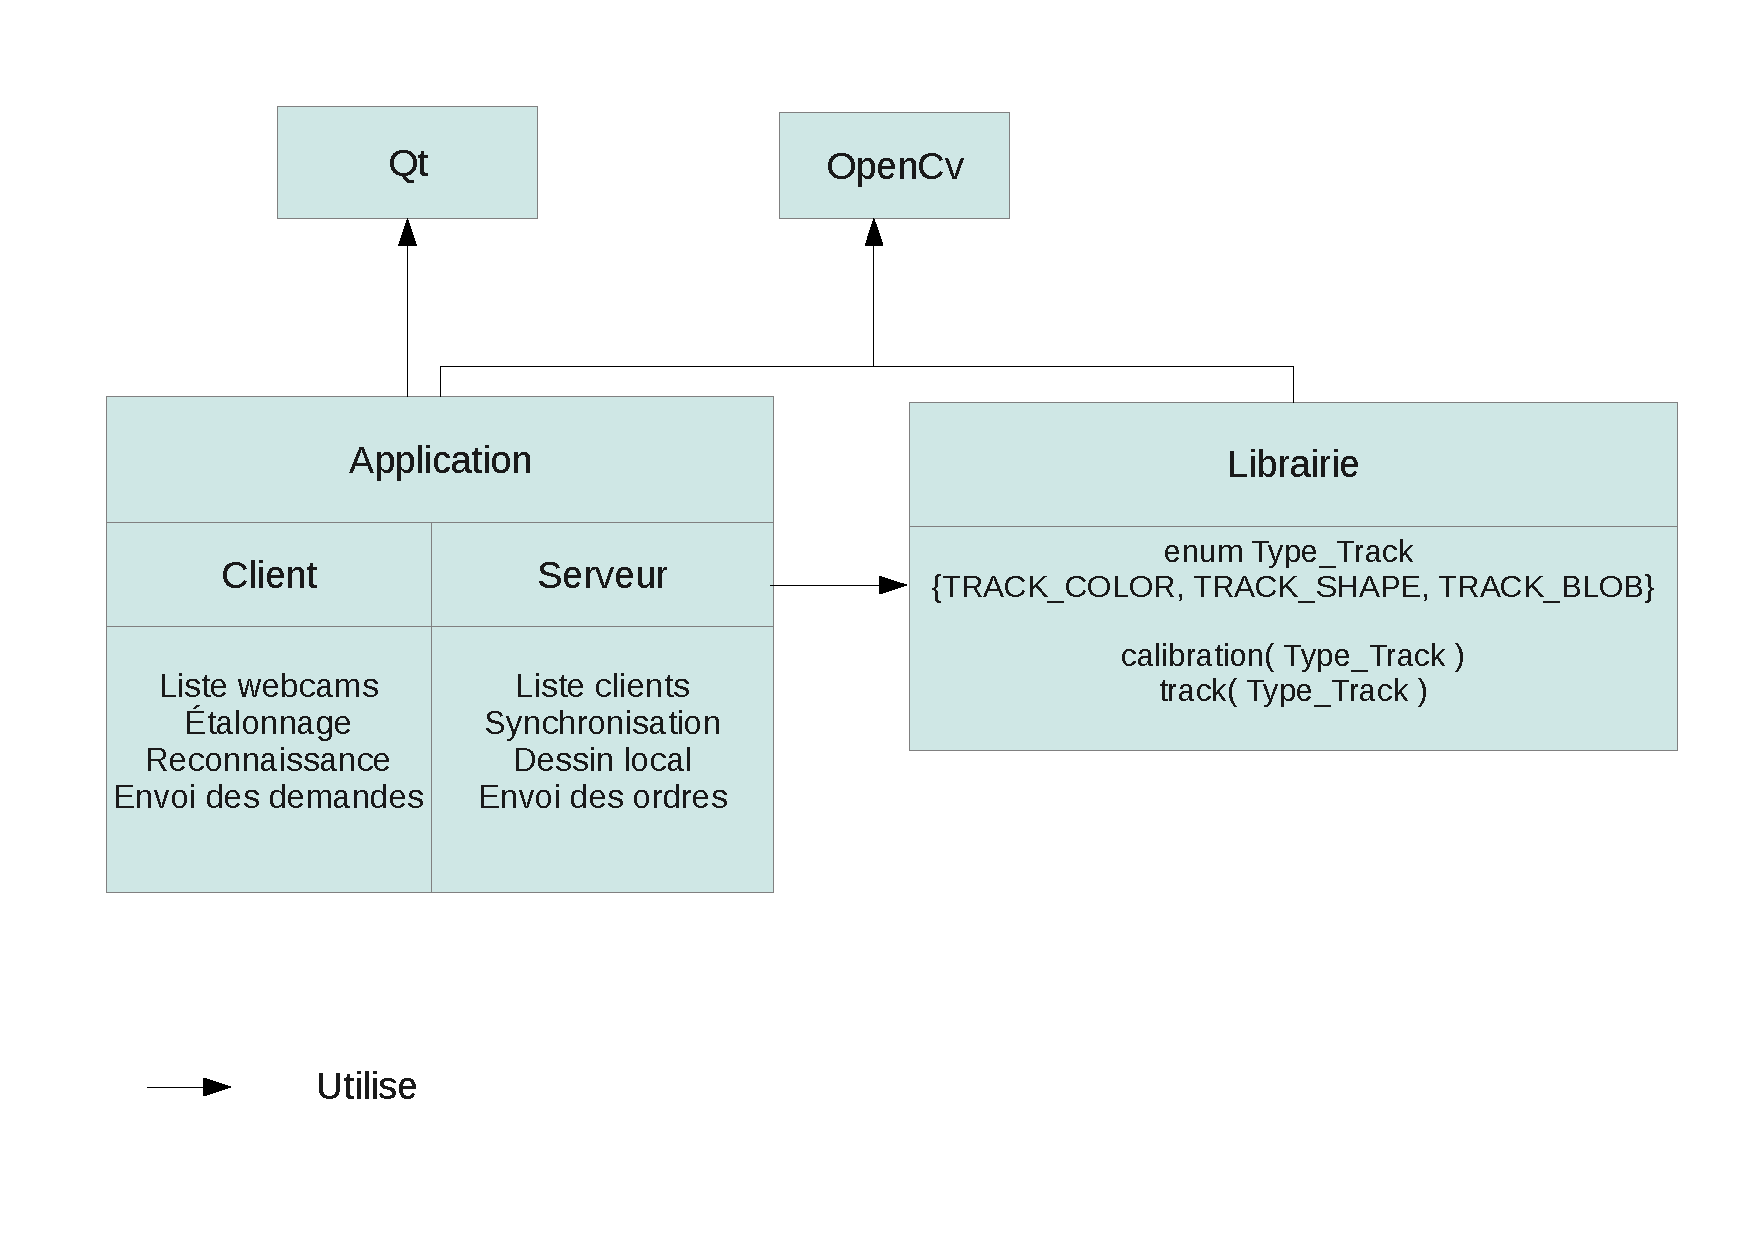
\includegraphics[scale=0.5]{schema_global.pdf}
	\end{center}
Le client et le serveur sont écrits à l'aide de la librairie Qt, et le client instancie la librairie pour reconnaître les mouvements. \\
La librairie utilise OpenCV pour le traitement de l'image et a pour but d'être réutilsable dans d'autres projets. 
Elle contient principalement une fonction d'étalonnage qui permet de signifier l'objet à suivre, ainsi que le type de suivi (Couleur, forme, avec cvBlob). La librairie possède ensuite un seul point d'entrée permettant d'effectuer le suivi.

\newpage
\section{Architecture de l'application}
L'application est conçue entièrement par dessus la librairie en essayant de minimimer le nombre de fonctions appellées. 
L'étalonnage du suivi de l'objet est effectué dans la classe $Calibration$, ensuite les appels pour suivre les mouvements sont faits
via une seule fonction dans la classe WidgetWebcam qui transmets ses mouvements au client (classe principale). \\

De plus l'application est conçue pour fonctionner de manière similaire pour une utilisation en réseau, ou en local, les classes 
représentant le tableau en local ou en réseau ont donc la même apparence (mêmes points d'entrées) vu de l'extérieur. \\
	\begin{center}
	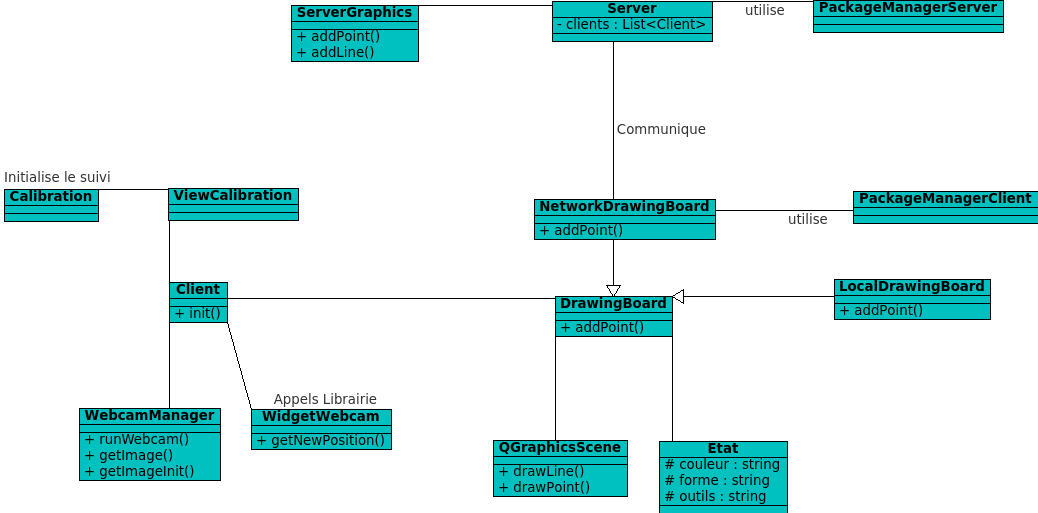
\includegraphics[scale=0.7]{../uml/classes.png}
	\end{center}

\section{Schéma lors d'une utilisation en réseau}
Ce schéma présente un déroulement des opérations lors d'une connexion et d'un dessin en utilisant les fonctionnalités réseaux.\\

\begin{itemize}
	\item Le client se connecte
	\item Le client effectue son étalonnage
	\item Le serveur l'enregistre, et lui envoie le tableau courant (vide ou non)
	\item Le client stocke le tableau et commence à détecter un mouvement
	\item Il envoie le mouvement détecté
	\item Le serveur reçoit le mouvement, dessine en local et renvoie à tous les clients l'ordre de dessin
	\item Le client reçoit l'ordre et dessine en local
\end{itemize}

\begin{center}
	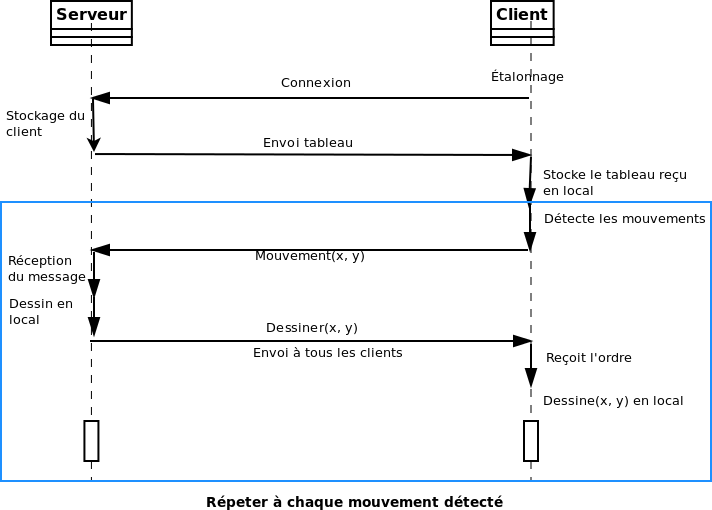
\includegraphics[scale=0.5]{../uml/sequence_reseau.png}
\end{center}

\end{document}

